\section{实现}
\label{kvdirect:sec:implementation}



本文的硬件平台基于基于英特尔Stratix V FPGA的可编程网卡(\S \ref {kvdirect:sec:programmable-nic})。
可编程网卡通过分叉x16物理连接器中的两个PCIe Gen3 x8链路连接到服务器,并包含4 GiB板载DRAM和一个DDR3-1600通道。

为了提高开发效率,使用英特尔FPGA SDK for OpenCL~ \cite {aoc}来合成OpenCL的硬件逻辑。
键值处理器采用1.1万行OpenCL代码实现,所有内核都完全流水线化,即吞吐量是每个时钟周期一次操作。
凭借180~MHz的时钟频率,可以在180~M op / s下处理键值操作,如果不是网络,DRAM或PCIe的瓶颈。
%
%\begin{table}[htbp]
%	\centering
%	\caption{Line of code and resource utilization of the 键值 processor.}
%	\label{kvdirect:tab:resource-util}
%	\scalebox{0.8}{
%		\begin{tabular}{l|r|r|r}
%			\toprule
%			Component & LoC & Logic (\%) & Memory (\%) \\
%			\midrule
%            Hash table & & & \\
%            Slab memory allocator & & & \\
%            Dynamic operation scheduler & & & \\
%            DRAM load dispatcher & & & \\
%            Operation decoder & & & \\
%            \midrule
%            Interconnect & & & \\
%            OpenCL runtime & & & \\
%            Network hard IP & & & \\
%            PCIe DMA and hard IP & & & \\
%            DDR controller & & & \\
%            \midrule
%            Total & & & \\
%			\bottomrule
%		\end{tabular}
%	}
%\end{table}

下面讨论几个实现中的细节。


\begin{figure}[t]
\centering
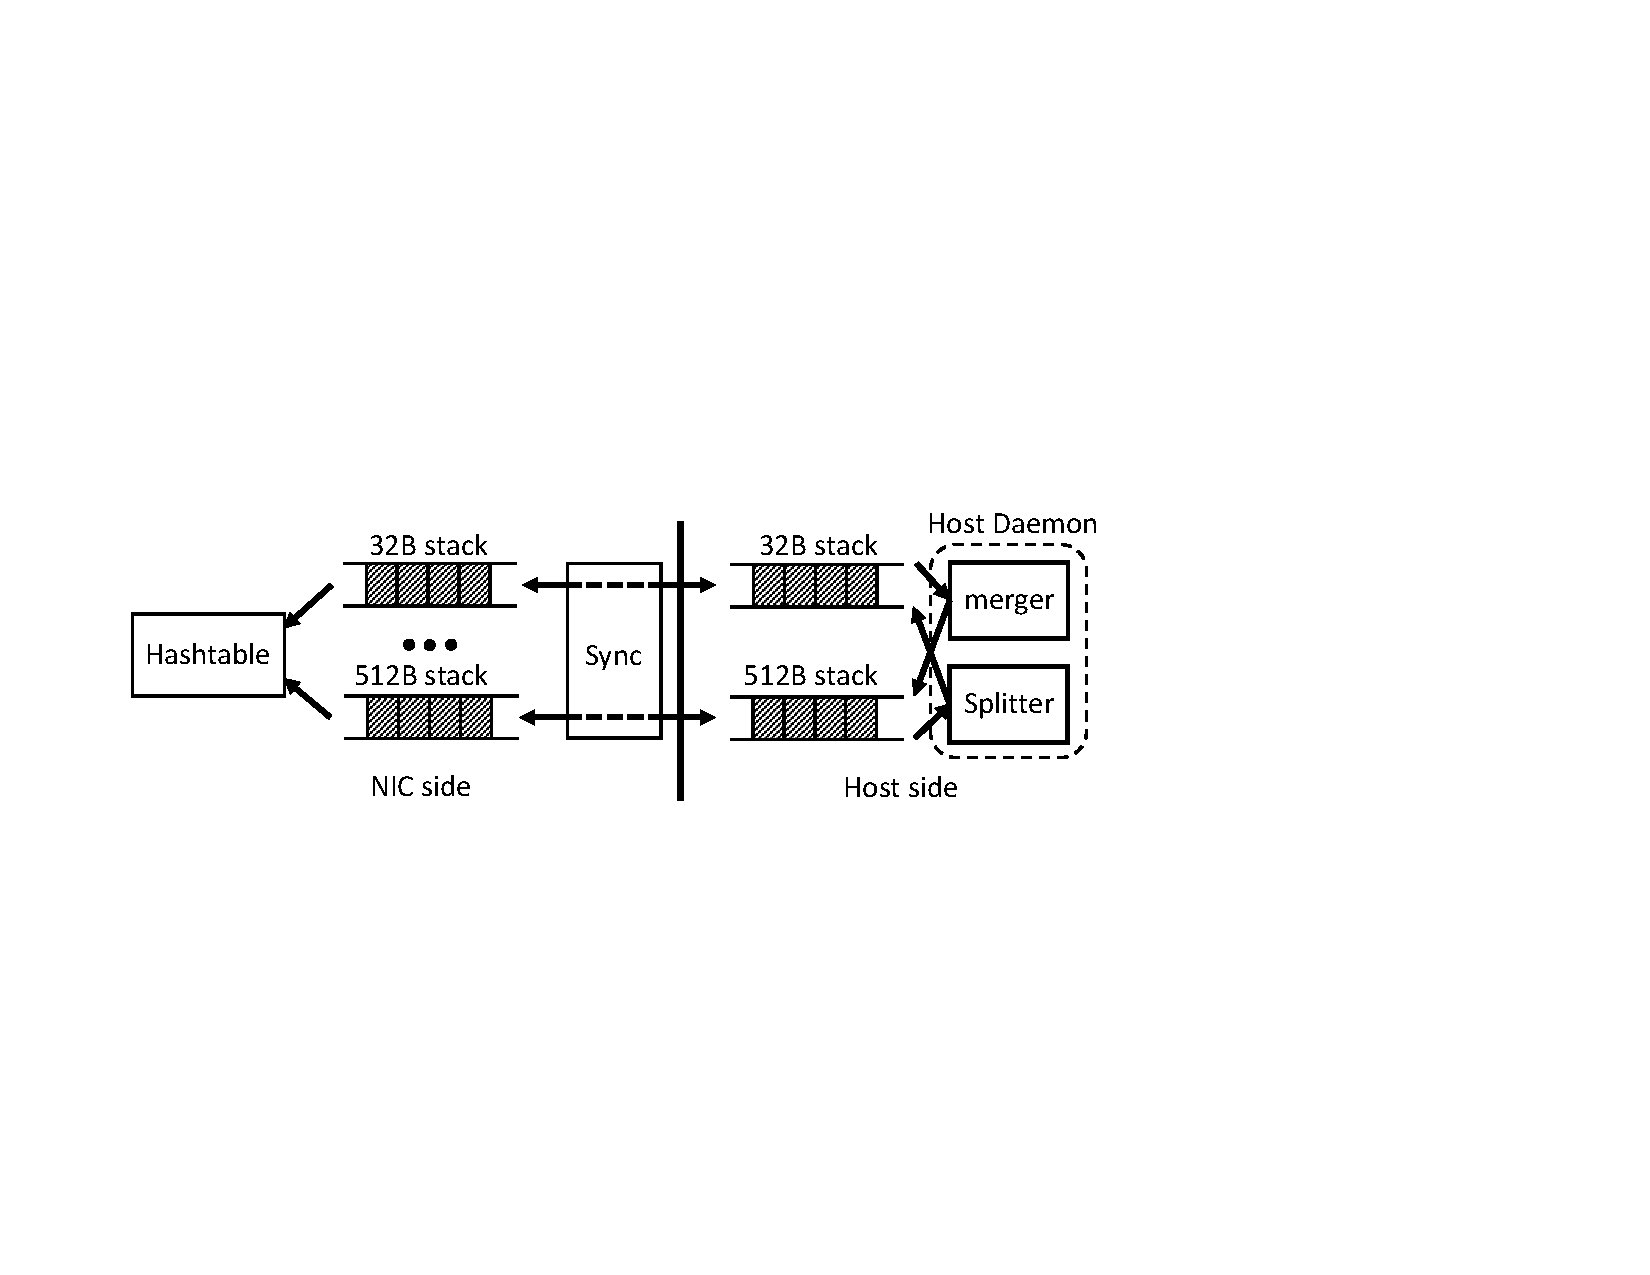
\includegraphics[width=.8\textwidth,page=1]{figure/cropped_slab.pdf}
\caption{Slab 内存分配器。}
\label{kvdirect:fig:slab}

\end{figure}

\subsection{Slab 内存分配器}
如图\ref {kvdirect:fig:slab}所示,对于每个slab大小,网卡上的slab缓存使用两个双端堆栈与主机DRAM同步。
对于网卡端双端堆栈(图\ref {kvdirect:fig:slab}中的左侧),左端由分配器和解除分配器弹出并推送,右端与左端同步通过DMA对应的​​主机端堆栈。
网卡监视网卡堆栈的大小,并根据高水位线和低水位线与主机堆栈同步。
主机守护进程定期检查主机端双端堆栈的大小。如果它高于高水印,则触发平板合并;当它低于低水印时,会触发平板分裂。
因为堆栈的每一端都是由网卡或主机访问的,并且在移动指针之前访问数据,所以不会发生竞争条件。

在本文中,每个slab条目是5个字节,DMA粒度是64个字节,因此每个slab操作的摊销DMA开销是$ 5/64 $。此外,当后续分配重新使用新释放的slab槽时,使用网卡上的堆栈而不是DMA。


\subsection{DRAM 负载均衡器}

一个技术挑战是在DRAM高速缓存中存储元数据,这需要额外的4个地址位和每64字节高速缓存行一个脏标志。
不需要缓存有效位,因为所有键值存储存储都由网卡专门访问。
为了存储每个高速缓存行的5个元数据位,将高速缓存行扩展到65个字节会由于未对齐访问而降低DRAM性能;将元数据保存在别处会使内存访问倍增。
相反,本文利用ECC DRAM中的备用位来进行元数据存储。
ECC DRAM通常每64位数据具有8个ECC位。
对于汉明码来纠正64位数据中的一位错误,只需要7个附加位。
第8个ECC位是用于检测双位错误的奇偶校验位。
当以64字节粒度和对齐方式访问DRAM时,每64B数据有8个奇偶校验位。
本文将奇偶校验检查粒度从64个数据位增加到256个数据位,因此仍然可以检测到双位错误。这允许了6个额外的位,可以保存地址位和脏标志。

%\textbf{键值 Operation Decoder.}
%The 键值 operation decoder saves receive timestamp and UDP flow tuple as execution context in reservation station.
%When the 键值 operation completes, the flow control component measures the processing delay from the receive timestamp in execution context.
%The network encoder needs the flow tuple to generate completion packets and send to the client.
%To avoid head-of-line blocking, 键值 operations are processed out-of-order, so the client may receive 键值 completions in a different order from requests.
%The client could match the completions with requests by the key, because completions with a same key are guaranteed to be in request order.

\subsection{向量操作译码器}
在整个键值处理器设计中,将批处理视为在一个存储桶中获取多个散列槽,使自由slab队列与主机内存同步,懒惰拆分和slab槽合并以及依赖键值操作的数据转发的通用原则。
批处理通过将控制平面开销分摊到多个数据平面有效负载来提高性能。
与PCIe相比,网络是一种更加稀缺的资源,具有更低的带宽(5~GB / s)和更高的延迟(2~$\mu$s)。
以太网上的RDMA写数据包有88字节的报头和填充开销,而PCIe TLP数据包只有26字节的开销。
这就是以前基于FPGA的键值存储 \cite{blott13hotcloud,blott2015scaling} 没有使PCIe带宽饱和的原因,尽管它们的哈希表设计效率低于KV-Direct。
这需要在两个方面进行\textit {客户端批处理}:在一个数据包中批量处理多个键值操作,并支持向量操作以实现更紧凑的表示。为此,在键值引擎中实现了一个解码器,从单个RDMA数据包中解压缩多个键值操作。
观察到许多键值具有相同的大小或重复值,键值格式包括两个标志位以允许复制密钥和值大小,或者包中的先前键值的值。
幸运的是,许多重要的工作负载(\textit {例如图遍历,参数服务器})可以批量发布键值操作。
展望未来,如果可以使用更高带宽的网络,则无需批量处理。
